\documentclass[a4paper,12pt]{article} % тип документа

% Поля страниц
\usepackage[left=2.5cm,right=2.5cm,
    top=2cm,bottom=2cm,bindingoffset=0cm]{geometry}
    
%Пакет дял таблиц   
\usepackage{multirow} 
    
%Отступ после заголовка    
\usepackage{indentfirst}

% Математика
\usepackage{floatrow}
\floatsetup[table]{style=Plaintop}

% \usepackage{hyperref}
\usepackage[warn]{mathtext} %позволяет добавлять кириллицу в формулы

\usepackage{amsmath,amsfonts,amssymb,amsthm,mathtools} 
\usepackage{wasysym}
\usepackage[warn]{mathtext}
\usepackage{multicol}
\usepackage{graphicx}
\usepackage[shortcuts,cyremdash]{extdash}
\usepackage{wrapfig} % обтекание текстом
\usepackage{floatflt}
\usepackage{lipsum}
\usepackage{verbatim}
\usepackage{xcolor}
\usepackage{etoolbox}
\usepackage{subfiles}
\usepackage{enumitem}
\usepackage{amsthm}

% Рисунки
\usepackage{floatrow,graphicx,calc}
\usepackage{wrapfig}

%%% Работа с картинками
\usepackage{graphicx}  % Для вставки рисунков
\graphicspath{{images/}{images2/}}  % папки с картинками
\setlength\fboxsep{3pt} % Отступ рамки \fbox{} от рисунка
\setlength\fboxrule{1pt} % Толщина линий рамки \fbox{}
\usepackage{wrapfig} % Обтекание рисунков и таблиц текстом

\renewcommand{\arctan}{\mathop{\mathrm{arctg}}\nolimits}
\newcommand{\divisible}{\mathop{\raisebox{-2pt}{\vdots}}}
\newcommand{\grad}{\mathop{\mathrm{grad}}\nolimits}
\newcommand{\diver}{\mathop{\mathrm{div}}\nolimits}
\newcommand{\rot}{\mathop{\mathrm{rot}}\nolimits}
\newcommand{\veci}{{\vec\imath}}                % i-орт
\newcommand{\vecj}{{\vec\jmath}}                % j-орт
\newcommand{\veck}{{\vec{k}}}                   % k-орт
\renewcommand{\phi}{\varphi}                    % Красивая фи
\newcommand{\der}[2]{\frac{d #1}{d #2}} % derivative
\newcommand{\dpart}[2]{\frac{\partial #1}{\partial #2}} % first partial der
\newcommand{\ddpart}[2]{\frac{\partial^2 #1}{\partial #2^2}} % вторая частная производная
\newcommand{\e}{\mathop{\mathrm e}\nolimits}    % Экспонента
\newcommand{\E}{\mathcal{E}}                    % ЭДС
\renewcommand{\epsilon}{\varepsilon}            % Красивый эпсилон
\newcommand{\degr}{\ensuremath{^\circ}}         % Градус
\newcommand{\const}{\text{const}} % постоянная
\newcommand{\Int}{\int\limits}          % Большой интеграл (можно поменять \int на \varint)
\newcommand{\IInt}{\iint\limits}          % Большой интеграл (можно поменять \int на \varint)
\newcommand{\Oint}{\oint\limits}                % Большой интеграл
\newcommand{\lvec}[1]{\overrightarrow{#1}}            % beauty vector arrow
\newcommand{\quot}[1]{<<#1>>}                   % russian quotes
\newcommand{\iu}{\imath}
\newcommand{\system}[1]{\left\lbrace\begin{array}{c} #1 \end{array} \right.}
\newcommand{\orsys}[1]{\left[\begin{array}{c} #1 \end{array} \right.}

\newcommand{\cvec}[1]{\left[\begin{array}{c} #1 \end{array} \right]}
\newcommand{\matr}[2]{\left(\begin{array}{#1} #2 \end{array} \right)}
\newcommand{\matrtwo}[1]{\matr{c c}{#1}}
\newcommand{\matrthree}[1]{\matr{c c c}{#1}}
\newcommand{\detmat}[2]{\left|\begin{array}{#1} #2 \end{array} \right|}
\newcommand{\dettwo}[1]{\detmat{c c}{#1}}
\newcommand{\detthree}[1]{\detmat{c c c}{#1}}
\newcommand{\gath}[1]{\begin{gathered} 	#1	\end{gathered}}

\newcommand{\mean}[1]{\langle #1 \rangle}

\newcommand{\RomanNumeralCaps}[1] {\MakeUppercase{\romannumeral #1}}

% Создаёем новый разделитель
\DeclareFloatSeparators{mysep}{\hspace{1cm}}

% Ссылки?
\usepackage{hyperref}
\usepackage[rgb]{xcolor}
\hypersetup{				% Гиперссылки
    colorlinks=true,       	% false: ссылки в рамках
	urlcolor=blue          % на URL
}


%  Русский язык

\usepackage[T2A]{fontenc}			% кодировка
\usepackage[utf8]{inputenc}			% кодировка исходного текста
\usepackage[english,russian]{babel}	% локализация и переносы
\usepackage[left=15mm,
            top=20mm,
            right=15mm,
            bottom=15mm,
            includefoot,
            footskip=10mm]{geometry} % настройки полей документа





% Математика
\usepackage{amsmath,amsfonts,amssymb,amsthm,mathtools}

%%% Дополнительная работа с математикой
\usepackage{amsmath,amsfonts,amssymb,amsthm,mathtools} % AMS
\usepackage{icomma} % "Умная" запятая: $0,2$ --- число, $0, 2$ --- перечисление


% Что-то 
\usepackage{wasysym}


\begin{document}

\begin{center}   
	\large{Лабораторная работа № 5.1.2\\\large{\textbf{Исследование эффекта Комптона}}}\\
		Аль Мажариш Гасем\\
		Группа Б01-202а
\end{center}

\thispagestyle{empty}

\section * {Цель работы}
С помощью сцинтилляционного спектрометра исследуется энергетический спектр $\gamma$-квантов, рассеянных на графите. Определяется энергия рассеянных $\gamma$-квантов в зависимости от угла рассеяния, а также энергия покоя частиц, на которых происходит комптоновское рассеяние.

\section * {Теоретические сведения}

Эффект Комптона — увеличение длины волны рассеянного излучения по сравнению с падающим — интерпретируется как результат упругого соударения двух частиц: $\gamma$-кванта (фотона) и свободного электрона. Волновая теория испытывает трудности при описании эффекта Комптона, поэтому в данном случае удобно считать электрон и $\gamma$-квант частицами, а их взаимодействие - упругим соударением. Запишем законы сохранения энергии и импульса для рассматриваемого явления:

\[ mc^2 + \hbar \omega_0 = \gamma mc^2 + \hbar \omega_1 \]
\[ dfrac{\hbar \omega_0}{c} = \gamma mv \cos{\varphi} + \dfrac{\hbar \omega_1}{c} \cos{\theta} \]
\[ \gamma mv \sin{\varphi} = \dfrac{\hbar \omega_1}{c} \sin{\theta} \]

Решая совместно эти уравнения и переходя от частот к длинам волн, получаем изменение длины рассеянного излучения
\begin{equation}
    \triangle \lambda = \lambda_1 - \lambda_0 = \frac{h}{mc}(1 - \cos \theta) = \Lambda_k(1 - \cos \theta),
\end{equation}
где $\Lambda_k = \frac{h}{mc} = 2.42 \dot 10^{-10}$ см - комптоновская длина волны электрона. \par
Основной целью работы является проверка соотношения (1). Преобразуем его от длин волн к энергии $\gamma$-квантов:
\begin{equation}
    \frac{1}{\varepsilon(\theta)} - \frac{1}{\varepsilon_0} = 1 - \cos \theta,
    \label{eq:Комптон_нормир}
\end{equation}
где $\varepsilon_0 = E_0/(mc^2)$ - энергия $\gamma$-квантов, падающих на рассеиватель (в единицах $mc^2$), $\varepsilon(\theta)$ - выраженная в тех же единицах энергия квантов, испытавших комптоновское рассеяния на угол $\theta$, $m$ - масса электрона.

\begin{figure}[h!]
    \centering
    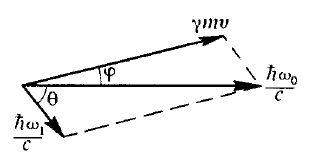
\includegraphics[width=0.5\linewidth]{fig1.PNG}
    \caption{Схема эффекта Комптона. Источник: [3]]}
    \label{fig:enter-label}
\end{figure}

\section * {Оборудование и инструментальные погрешности}

Источником излучения служит $^{137}$Cs(1), испускающий  $\gamma$-кванты с энергией 662 кэВ. Узкий пучок после коллиматора попадает на графитовую мишень (2). Кванты, испытавшие комптоновское рассеяния в мишени, регистрируются сцинтилляционным счетчиком и проходят на ФЭУ. Сигналы, возникающие на ФЭУ, подаются на ЭВМ для амплитудного анализа. Штанга с измерительным блоком может вращаться относительно мишени.

        \begin{figure}[h]
\begin{center}
\begin{minipage}[h]{0.48\linewidth}
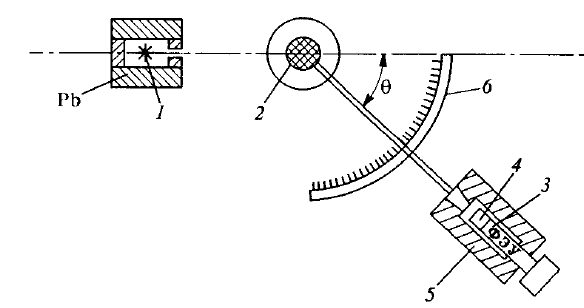
\includegraphics[width=1\linewidth]{fig2.PNG}
\caption{Схема установки. Источник: [3]} 
\end{minipage}
\hfill 
\begin{minipage}[h]{0.48\linewidth}
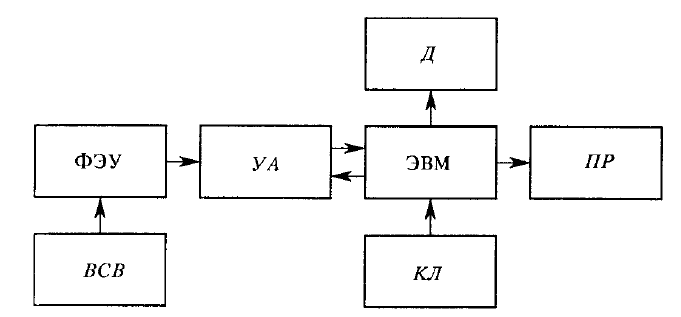
\includegraphics[width=1\linewidth]{fig3.PNG}
\label{ris:experimcoded}
\end{minipage}
\end{center}
\end{figure}


\section * {Результаты измерений и обработка данных}
\subsection * {Расчёт значений}

Устанавливая сцинтилляционный счётчик под разными углами $\theta$ к первоначальному направлению полета $\gamma$-квантов, получим амплитудные спектры и определим положения фотопиков на них. 

Запишем формулу \eqref{eq:Комптон_нормир} в удобном виде:
	\begin{equation}\label{eq:Комптон_число}
		\dfrac{1}{N(\theta)} - \dfrac{1}{N(0)} = 1- \cos(\theta).
	\end{equation}
	Здесь $ N(\theta) $ -- номер канала.

 Теперь построим график, откладывая $(1 - \cos{\theta})$ по оси абсцисс, а $\dfrac{1}{N(\theta)}$ по оси ординат.

 \begin{figure}[h!]
     \centering
     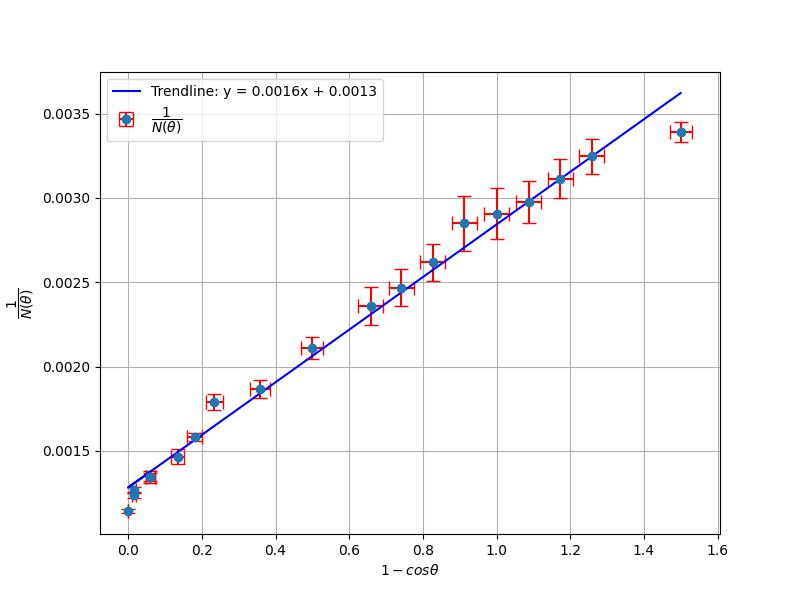
\includegraphics[width=1\linewidth]{plot.jpg}
     \caption{Зависимость $\dfrac{1}{N(\theta)}$ от $1 - \cos{\theta}$}
     \label{fig:plot}
 \end{figure}

Как видно из графика, качественно результаты сходятся с теорией и зависимость действительно соответствует прямой:

\[y = (0.0016\pm 0.00005)\times x + (0.0013\pm 0.00001)\]
\[N_{наил}(0) = 769 \pm 6\]
\[N_{наил}(90^\circ) = 344\pm 5\]
	
Исходя из этих данных определим энергию покоя частицы, на которой происходит комптоновское рассеяние (по всем признакам -- электрон):
\[m c^2 = E_\gamma \dfrac{N(90^\circ)}{N(0)-N(90^\circ)} = 0.536 \text{МэВ}\]

\subsection * {Расчёт погрешностей}

Погрешность угла примем $\Delta \theta = 2 ^ \circ$, $\Delta N$ будем оценивать после каждого измерения. Для получения крестов погрешности воспользуемся формулой:

\[\Delta f(x) = |f'(x)| \times \Delta x\]

Тогда:

\[\Delta \cos{\theta} = |\sin{\theta} \times \Delta \theta|\]
\[ \Delta \dfrac{1}{N(\theta)} = \dfrac{\Delta N}{N^2}\]

Оценим погрешность выражения энергии покоя электрона как погрешность частного с абсолютными погрешностями $\Delta N(90 ^ \circ)$ и $(\Delta N(90 ^ \circ) + \Delta N(0))$.

\[ \epsilon \geq \dfrac{\Delta N(90 ^ \circ)}{N(90 ^ \circ)} + \dfrac{\Delta N(90 ^ \circ) + \Delta N(0)}{N(0) - N(90 ^ \circ)}\] = 0.04

следовательно

\[ mc^2 = (0.536 \pm 0.021) \text{МэВ} \]

Что, хоть и не совпадает с табличными данными в пределах погрешности, но очень близко к ним.


\section * {Вывод}

По результатам работы, исследовали эффект Комптона на графитовом образце с помощью сцинтилляционного спектрометра. Выяснили зависимость  энергии рассеянного \gmm-кванта от угла рассеяния, а также определили по порядку величины энергию покоя электрона. \\

При подсчёте энергии покоя электрона получили несовпадение с табличными данными, скорее всего это из-за заниженной погрешности, что, в свою очередь, является следствием оценки погрешности канала "на глаз".



\begin{thebibliography}{9}
	\bibitem{Siv} Сивухин Д. В. \emph{Общий курс физики. Том 5 Атомная и ядерная физика}, 2004
	\bibitem{kir} Кириченко Н. А. \emph{Начальные главы квантовой механики}, 2014
	\bibitem{max} \emph{Лабораторный практикум по общей физике. Квантовая физика.} под ред. Ю. М. Ципенюка
\end{thebibliography}
\end{document}

















